\documentclass{article}
\usepackage[a4paper,
total={6.5in, 10in},
voffset=5px]{geometry}
\usepackage{fancyhdr}
\usepackage[fleqn]{amsmath}
\usepackage{titling}
\usepackage[shortlabels]{enumitem}
\usepackage{amsthm}
\usepackage{amssymb}
\usepackage[bb=boondox]{mathalfa}
\usepackage{ifthen}
\usepackage{amsfonts}
\usepackage{algorithm}
\usepackage{algpseudocode}
\usepackage{indentfirst}
\usepackage{tikz}
\usepackage{tkz-graph}
\usepackage{float}
\usepackage{hyperref}
\usepackage{cleveref}
\usepackage{MnSymbol}
\usepackage{ifthen}
\usepackage{listings}
\usepackage{bussproofs}
\usepackage{lineno}
\usepackage{multicol}

\linenumbers

\renewcommand\linenumberfont{\normalfont\small\sffamily}
\fontfamily{qcr}\selectfont

\usetikzlibrary{positioning}

\hypersetup{
  colorlinks=true,
  allcolors=blue,
}

% \pagestyle{fancy}

\algnewcommand\algorithmicinput{\textbf{Input:}}
\algnewcommand\Input{\item[\algorithmicinput]}
\algnewcommand\algorithmicoutput{\textbf{Output:}}
\algnewcommand\Output{\item[\algorithmicoutput]}
\algnewcommand\Ret[1]{\State \textbf{return }$#1$ }
\algnewcommand\Clarif{\item[\textbf{Clarification: }]}
\algnewcommand\Assign[2]{\State $#1 = #2$}

\algnewcommand \Foreach[3]{\For{$#1 \textbf{ in } #2$}
  #3
  \EndFor
}

\algnewcommand \IIf[2]{\If{$#1$}
  #2
  \EndIf}

\algnewcommand \IIfE[3]{\If{$#1$}
  #2
  \Else
  #3
  \EndIf}

\algnewcommand \Func[3]{\Function{#1}{#2}
  #3
  \EndFunction}

\algnewcommand \Whl[2]{
  \While{$#1$}
  #2
  \EndWhile
}

\algrenewcommand\textproc{}
\newcommand{\LineComment}[1]{\\/*\textit{#1}\hfill*/}

\definecolor{codegreen}{rgb}{0,0.6,0}
\definecolor{codegray}{rgb}{0.5,0.5,0.5}
\definecolor{codepurple}{rgb}{0.58,0,0.82}
\definecolor{backcolour}{rgb}{0.95,0.95,0.92}

\lstdefinestyle{mystyle}{
    backgroundcolor=\color{backcolour},   
    commentstyle=\color{codegreen},
    keywordstyle=\color{magenta},
    numberstyle=\small\color{codegray},
    stringstyle=\color{codepurple},
    breaklines=true,                 
    captionpos=b,                    
    numbers=left,                    
    numbersep=5pt,
    showspaces=false,                
    showstringspaces=false,
    showtabs=false,                  
    tabsize=4
}
\lstset{style=mystyle}

\newcommand{\axiom}[1]{\AxiomC{$#1$}}
\newcommand{\unary}[1]{\UnaryInfC{$#1$}}
\newcommand{\binary}[1]{\BinaryInfC{$#1$}}
\newcommand{\trinary}[1]{\TrinaryInfC{$#1$}}
\newcommand{\quaternary}[1]{\QuaternaryInfC{$#1$}}
\newcommand{\rlabel}[1]{\RightLabel{#1}}

\begin{document}
\pagenumbering{arabic}
I am now looking into algorithm typing of DOT and following are my thoughts from last
week. Let me know if you have suggestions. To summarize, my questions are following,
and details are broken down into further below.

\begin{enumerate}
\item Is it a good idea to unify record type and object type?
\item To handle subtyping, it does not seem straightforward to me to get around
  computing SCC. Is it good enough to assert ``facts'' about SCC, since it's well
  known? 
\item Up to which point is it sufficient in terms of handling and updating SCCs?
\end{enumerate}

Detailed discussions are following:

\begin{enumerate}
\item treatment of recursive type.

  In order to turn type judgment into an algorithm, we need to eliminate
  non-determinism to a point where there is only one rule for each context-term
  pair. Essentially, function with following signature is supposed.
  \begin{lstlisting}[language=Haskell]
    typeJudge :: Context -> Term -> Type
  \end{lstlisting}
  Potentially, this function should return the most precise type that can get from the
  context. 

  I find that following two judgments are especially problematic, since they can be
  applied to all terms.

  \nolinenumbers
  \begin{multicols}{2}
    \begin{prooftree}
      \axiom{\Gamma \vdash x : T}
      \rlabel{\textbf{(REC-I)}}
      \unary{\Gamma \vdash x : \mu(x : T)}
    \end{prooftree}

    \columnbreak
    \begin{prooftree}
      \axiom{\Gamma \vdash x : \mu(z : T)}
      \rlabel{\textbf{(REC-E)}}
      \unary{\Gamma \vdash x : [x/z]T}
    \end{prooftree}
  \end{multicols}

  \linenumbers I think one way to deal with these two is to remove them. My
  rationale is, the existence of two rules simply indicates the essential equivalence
  of any type and its recursive wrapper. But if I do this, there will be difficulties
  to handle object when a record is required, and the other way, even though any
  record type can only be instantiated by objects, and in reality, there really isn't
  fundamental difference between them. 

  Following this line of thought, it seems that unifying object type and record type
  is an option. However, that really means the model language will be changed. Do
  you think it's something OK to do? It sounds to me doing so becomes finding an
  alternative model language already. But if not doing so, it's not obvious to me
  that if there exists other algorithmic way to handle these two rules.

  One observation of looking to unifying these two types is, the type of resulting
  language will essential become top + bottom + structural refinement + lambdas +
  paths, which shows some similarities between both DOT and featherweight Scala. And
  we've known the latter has algorithmic typing.
  
\item subtyping.

  I feel some difficulties regarding this part as well. Following the similar path to
  step typing, I am thinking in terms of three functions for this part.

  \nolinenumbers
  \begin{lstlisting}[language=Haskell]
    isSubType :: Context -> Type -> Type -> Bool
    exposure :: Context -> Type -> Type
    promote :: Context -> Var -> Type -> Type
  \end{lstlisting}

  \linenumbers
  The motivation of thinking of these two functions, following the same path of step
  typing, is to reformulate following rules.

  \begin{prooftree}
    \axiom{\Gamma \vdash x : T'}
    \axiom{(exposure\ \Gamma\ T') = \forall(z : S)T}
    \axiom{\Gamma \vdash y : S'}
    \axiom{isSubType\ \Gamma\ S'\ S}
    \rlabel{\textbf{(ALL-E)}}
    \quaternary{\Gamma \vdash x\ y : [y/z]T}
  \end{prooftree}

  \begin{prooftree}
    \axiom{\Gamma \vdash t: T}
    \axiom{\Gamma, x : T \vdash u: U}
    \rlabel{\textbf{(LET)}}
    \binary{\Gamma \vdash let\ x = t\ in\ u: (promote\ (\Gamma, x : T)\ x\ U)}
  \end{prooftree}

  However, regardless of whether we change the model language or not, there is a cycle
  issue among subtypes. So I think SCC at minimum is necessary. But some search shows
  that even implementing DFS would not be
  trivial. \url{http://gallium.inria.fr/~fpottier/publis/fpottier-dfs-scc.pdf} this
  paper shows DFS as a function, but not yet reach SCC. Even though one exists,
  properties involving SCC might not be straightforward. Are you aware how people do
  formalization with cycle detection? Is it OK to assert axioms to get away with
  proving those well-known properties of SCC?

\item maintaining SCC.

  Thinking ahead, I am trying to obtain a big picture of how the graph representing
  subtype relation should be maintained. I am think of following two (dual) functions
  in order to define \textbf{exposure} and \textbf{promote}:

  \nolinenumbers
  \begin{lstlisting}[language=Haskell]
    -- |the supertype of all types that are subtypes of two input types.
    supremum :: Context -> Type -> Type -> Type
    -- |the subtype of all types that are supertypes of two input types.
    infimum :: Context -> Type -> Type -> Type 
  \end{lstlisting}

  \linenumbers
  To do this, I imagine whenever an object type is pushed into the typing context, the
  graph needs to be updated, and the function \textbf{exposure} and \textbf{promote}
  will rely on the graph. I am thinking of the update in terms of following steps(an
  edge $U \to V$ indicates $U <: V$ in the context).

  \nolinenumbers
  \begin{algorithm}[H]
    \caption{graph update algorithm}
    \begin{algorithmic}[1]
      \Foreach{\{A : S..T\}}{\mu(x : \{...\})}{
        \State{add $S \to x.A$, $x.A \to T$ to the graph}
      }
      \State{run SCC on the new graph}
      \LineComment{following step guarantees every path type has a concrete type as
        its infimum and supremum for every SCC.}
      \Foreach{\text{(weakly) connected SCC subgraph}}{\text{SCC graphs}}{
        \State{add edges from $\top$ to the sources that are a path type}
        \State{add edges to $\bot$ from the sinks that are a path type}
      }
    \end{algorithmic}
  \end{algorithm}

  \linenumbers
  The second for loop is to handle those object types which purely introduce cycles.

  \nolinenumbers
  \begin{multicols}{2}
    \begin{lstlisting}[language=Haskell, mathescape=true]
      $\mu$ x : {
        A : x.B .. x.C
        B : x.C .. x.A
        C : x.A .. x.B
      }
    \end{lstlisting}

    \columnbreak
    \begin{figure}[H]
      \centering
      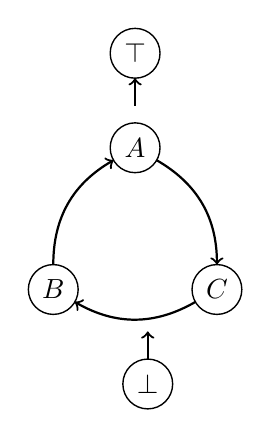
\begin{tikzpicture}
        \SetGraphUnit{1.2}
        \SetVertexMath
        \tikzset{EdgeStyle/.append style={->}}

        \begin{scope}[rotate=90]
          \Vertices{circle}{A, B, C}
        \end{scope}

        \NO[L=\top](A){top}
        \SOEA[L=\bot](B){bot}

        \node[above=10pt of bot](bott){};
        \Edge(bot)(bott)

        \node[below=10pt of top](topp){};
        \Edge(topp)(top)

        \tikzset{EdgeStyle/.append style={bend left}}
        \Edges(A, C, B, A)
      \end{tikzpicture}
    \end{figure}
  \end{multicols}

  \linenumbers
  Here, the cycle collapse all these three types into a single one, and they can be
  assigned to any types. 

  I can think of two ways to handle each SCC.
  \begin{enumerate}
  \item Leave the SCC as it is. This in fact simulates what DOT actually does.
    However, since DOT is non-deterministic, it's unclear to me how to make
    \textbf{promote} or \textbf{exposure} deterministic and return the most
    ``desirable'' type. Also the cycle might contain inconsistency, like following.

    \nolinenumbers
    \begin{lstlisting}[language=Haskell, mathescape=true]
      $\mu$ x : {
        A : $\forall$(y: $\bot$)$\top$ .. $\mu$ z: { C : $\bot$ .. $\top$ }
        B : $\mu$ z: { C : $\bot$ .. $\top$ } .. $\forall$(y: $\bot$)$\top$
      }
    \end{lstlisting}
    \linenumbers
  \item One observation is, assuming no intersection type is involved, each SCC
    degenerates to simply typed lambda calculus with objects, and therefore
    unification seems possible with all path types treated as type
    variables. Therefore all non path types need to be syntactically compatible. This
    effectively tries hard to prove the type lattice remains familiar, after the
    subtype constraints are added.

    There are subtleties in this method as well. Since every unification will
    introduce new equations, after this, we need to keep doing unification with new
    equations until the number of SCCs stablizes, the termination of which is not
    obvious at all. It's more complex than simply require $S <: U$ being provable for
    each $\{A : S <: U\}$ like it's done in $D_{<:}$, due to the recursive nature of
    object type.
  \end{enumerate}

  It seems to me that this constraint resolution part will be big and with all these
  heavy dependencies on graph theory, I am not sure if it can be formalized in
  coq. Do you have better suggestions on how to approach it?

  Will it be beneficial to understand how dotty handles paths? For now, I am trying to
  look into order theory to get some inspiration.
  
  % In general, this graph must contains all path types involving any objects in the
  % typing context. Since the context is finite, and each object is finite, the graph
  % must be finite, and search in it must be decidable.

\item intersection type.

  I think intersection type is very difficult to handle, as it introduces too much
  non-determinism if intersection types involve path types. For example, it prevents
  unification like above from being possible.
  
  \nolinenumbers
  \begin{lstlisting}[language=Haskell, mathescape=true]
    $\mu$ x : {
      A : $\bot$ .. $\top$
      B : $\bot$ .. $\top$

      C : $x.A \wedge x.B$ .. $\mu$ x : { ... }
      D : $\mu$ x : { ... } .. $x.A \wedge x.B$ -- same object type as above
    }
  \end{lstlisting}

  \linenumbers
  It's entirely unclear what information can be retrieved from
  $x.A \wedge x.B \equiv \mu\ x : \{\ ...\ \}$. In this case, $x.A$ can be anywhere
  from $\top$ to all of $\mu\ x:\{\ ...\ \}$. More generally, for relation
  $A \wedge B <: C$, the only derivable relation from this is
  $A \wedge B <: A \wedge C$ and $A \wedge B <: B \wedge C$, which gives no better
  information than orginally. I think the interaction between intersection type and
  path type might become the source the undecidability, if one ever proves
  it. Considering all the previous problems are quite complex already, I am thinking
  leave this case. What do you think about this?
\end{enumerate}
\end{document}